\documentclass{beamer}
\mode<presentation>
\usepackage{amsmath,amssymb,mathtools}
\usepackage{textcomp}
\usepackage{gensymb}
\usepackage{adjustbox}
\usepackage{subcaption}
\usepackage{enumitem}
\usepackage{multicol}
\usepackage{listings}
\usepackage{url}
\usepackage{graphicx} % <-- needed for images
\def\UrlBreaks{\do\/\do-}

\usetheme{Boadilla}
\usecolortheme{lily}
\setbeamertemplate{footline}{
  \leavevmode%
  \hbox{%
  \begin{beamercolorbox}[wd=\paperwidth,ht=2ex,dp=1ex,right]{author in head/foot}%
    \insertframenumber{} / \inserttotalframenumber\hspace*{2ex}
  \end{beamercolorbox}}%
  \vskip0pt%
}
\setbeamertemplate{navigation symbols}{}

\lstset{
  frame=single,
  breaklines=true,
  columns=fullflexible,
  basicstyle=\ttfamily\tiny   % tiny font so code fits
}

\numberwithin{equation}{section}

% ---- your macros ----
\providecommand{\nCr}[2]{\,^{#1}C_{#2}}
\providecommand{\nPr}[2]{\,^{#1}P_{#2}}
\providecommand{\mbf}{\mathbf}
\providecommand{\pr}[1]{\ensuremath{\Pr\left(#1\right)}}
\providecommand{\qfunc}[1]{\ensuremath{Q\left(#1\right)}}
\providecommand{\sbrak}[1]{\ensuremath{{}\left[#1\right]}}
\providecommand{\lsbrak}[1]{\ensuremath{{}\left[#1\right.}}
\providecommand{\rsbrak}[1]{\ensuremath{\left.#1\right]}}
\providecommand{\brak}[1]{\ensuremath{\left(#1\right)}}
\providecommand{\lbrak}[1]{\ensuremath{\left(#1\right.}}
\providecommand{\rbrak}[1]{\ensuremath{\left.#1\right)}}
\providecommand{\cbrak}[1]{\ensuremath{\left\{#1\right\}}}
\providecommand{\lcbrak}[1]{\ensuremath{\left\{#1\right.}}
\providecommand{\rcbrak}[1]{\ensuremath{\left.#1\right\}}}
\theoremstyle{remark}
\newtheorem{rem}{Remark}
\newcommand{\sgn}{\mathop{\mathrm{sgn}}}
\providecommand{\abs}[1]{\left\vert#1\right\vert}
\providecommand{\res}[1]{\Res\displaylimits_{#1}}
\providecommand{\norm}[1]{\lVert#1\rVert}
\providecommand{\mtx}[1]{\mathbf{#1}}
\providecommand{\mean}[1]{E\left[ #1 \right]}
\providecommand{\fourier}{\overset{\mathcal{F}}{ \rightleftharpoons}}
\providecommand{\system}{\overset{\mathcal{H}}{ \longleftrightarrow}}
\providecommand{\dec}[2]{\ensuremath{\overset{#1}{\underset{#2}{\gtrless}}}}
\newcommand{\myvec}[1]{\ensuremath{\begin{pmatrix}#1\end{pmatrix}}}
\let\vec\mathbf

\title{MatGeo Presentation - Problem 4.7.61}
\author{EE25BTECH11064 - Yojit Manral}
\date{}

\begin{document}

\frame{\titlepage}
\begin{frame}{Question}
Find the coordinates of the foot of the perpendicular drawn from the origin to the plane $2x - 3y + 4z - 6 = 0$
\end{frame}

\begin{frame}{Solution}
$\rightarrow$ From the equation of a general plane,
\begin{align} \vec{n}^{T}\vec{x} = c \end{align}
$\rightarrow$ A vector perpendicular to the plane and passing through the origin can be given as \begin{align} \vec{y} = \alpha \vec{n} \end{align}
$\rightarrow$ The foot of perpendicular must be the intersection of (1) and (2)...
\begin{align}
    \vec{n}^{T} (\alpha \vec{n}) &= c \\
    \alpha \vec{n}^{T} \vec{n} &= c \\
    \alpha &= \frac{c}{\norm{\vec{n}}^{2}}
\end{align}
$\rightarrow$ Now we can find the foot of perpedicular as
\begin{align} \vec{x_\perp} = \alpha \vec{n} = \frac{c}{\norm{\vec{n}}^{2}} \vec{n} \end{align}
\end{frame}

\begin{frame}{Solution}
$\rightarrow$ Given that
\begin{align}
    \vec{n} = \myvec{2\\-3\\4} \implies \norm{\vec{n}}^{2} = 29 \text{  and  } c = 6 \\
    \implies \vec{x_\perp} = \frac{6}{29} \myvec{2\\-3\\4} = \myvec{12/29\\-18/29\\24/29}
\end{align}
\end{frame}
\begin{frame}{Solution}
\begin{figure}[h!]
   \centering
   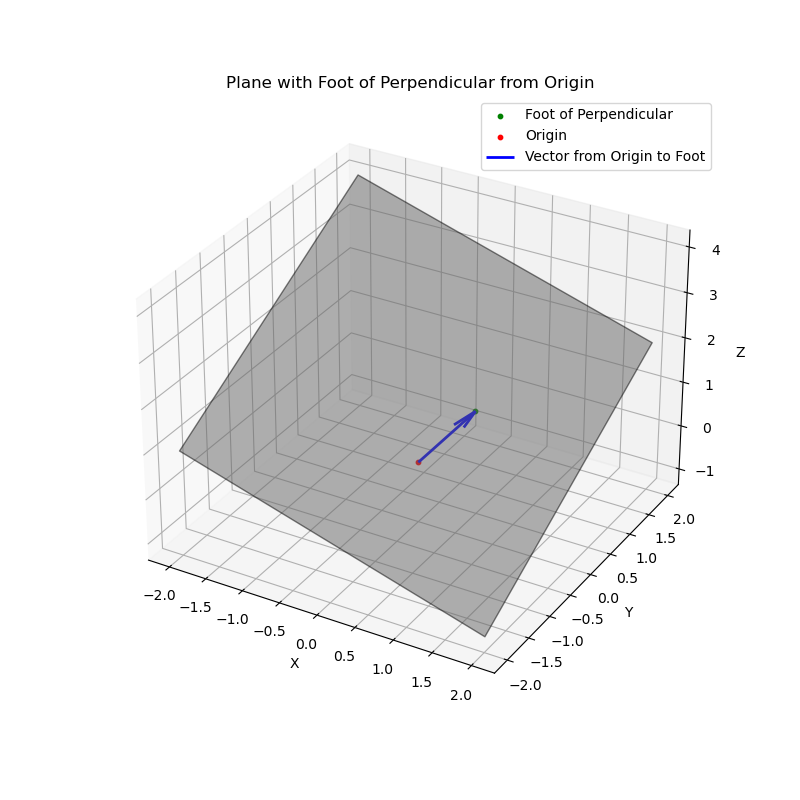
\includegraphics[width=0.6\linewidth]{figs/01.png}
   \caption{Foot of perpendicular of plane from origin}
   \label{Plot_1}
\end{figure}
\end{frame}
 % --------- CODE APPENDIX ---------
\section*{Appendix: Code}

% C program
\begin{frame}[fragile]{File: points.c}
\begin{lstlisting}[language=C]
#include <stdio.h>

int main() {
  FILE *fp;

  // -------------------
  // Question 4.7.61
  // -------------------


  fp = fopen("points.dat", "w");
  fprintf(fp, "%d,%d,%d\n", 2, -3, 4);  // n
  fclose(fp);
  return 0;
}
\end{lstlisting}
\end{frame}

% Python calling C
\begin{frame}[fragile]{File: call\_c.py}
\begin{lstlisting}[language=Python]
import subprocess

# Compile the C program
subprocess.run(["gcc", "points.c", "-o", "points"])

# Run the compiled C program
result = subprocess.run(["./points"], capture_output=True, text=True)

# Print the output from the C program
print(result.stdout)
\end{lstlisting}
\end{frame}

% Python plotting
\begin{frame}[fragile]{File: plot.py}
\begin{lstlisting}[language=Python]
import numpy as np
import matplotlib.pyplot as plt
from mpl_toolkits.mplot3d import Axes3D

# Plane equation: 2x - 3y + 4z - 6 = 0
# The point is the foot of the perpendicular (12/29, 18/29, 24/29)
foot_of_perpendicular = np.array([12/29, 18/29, 24/29])

# Create grid for the plane
x = np.linspace(-2, 2, 100)
y = np.linspace(-2, 2, 100)
X, Y = np.meshgrid(x, y)

# Solve for Z using the plane equation 2x - 3y + 4z - 6 = 0
Z = (6 - 2*X + 3*Y) / 4

# Create a 3D plot
fig = plt.figure(figsize=(8, 8))
ax = fig.add_subplot(111, projection='3d')

# Plot the plane
ax.plot_surface(X, Y, Z, alpha=0.5, rstride=100, cstride=100, color='gray', edgecolor='k')

# Plot the foot of the perpendicular
ax.scatter(foot_of_perpendicular[0], foot_of_perpendicular[1], foot_of_perpendicular[2], color='g', s=10, label='Foot of Perpendicular')
\end{lstlisting}
\end{frame}

% Python plotting
\begin{frame}[fragile]{File: plot.py}
\begin{lstlisting}[language=Python]
# Plot the origin
ax.scatter(0, 0, 0, color='r', s=10, label='Origin')

# Draw the vector from origin to foot of perpendicular
ax.quiver(0, 0, 0, foot_of_perpendicular[0], foot_of_perpendicular[1], foot_of_perpendicular[2], 
          color='b', linewidth=2, label='Vector from Origin to Foot')

# Labels and Title
ax.set_xlabel('X')
ax.set_ylabel('Y')
ax.set_zlabel('Z')
ax.set_title('Plane with Foot of Perpendicular from Origin')

# Show the plot
plt.legend()
plt.show()

\end{lstlisting}
\end{frame}

\end{document}
